\documentclass[12pt]{article}
\usepackage{amsmath}
\usepackage{graphicx,geometry}
\usepackage{array,url}
\usepackage[breaklinks]{hyperref}
\geometry{margin=1in}
\usepackage{setspace}
\usepackage{titling}
\setlength{\parskip}{0.5em}

\begin{document}
\begin{minipage}{0.45\textwidth}
  
\includegraphics[width=\linewidth]{Logo.png}
\end{minipage}
\hfill
\begin{minipage}{0.45\textwidth}
  \raggedleft
  \textbf{Name: Surabhi P}\\
  \textbf{Id: COMETFWC032}\\
  \textbf{Date: 29 August 2025}
\end{minipage}

\vspace{1cm}

\begin{center}
\fbox{
    \parbox{0.9\textwidth}{
       \centering
       \small

       \url{https://github.com/surabhi84ard/Mini/tree/8e9042b13304f4b4923d330711d1eb424065bccb/avr-gcc}
    }
}

    {\LARGE \textbf{GATE Question solution using Avr-gcc}}\\[1em]
\end{center}

\section*{Question}


\begin{figure}[h!]
    \centering
    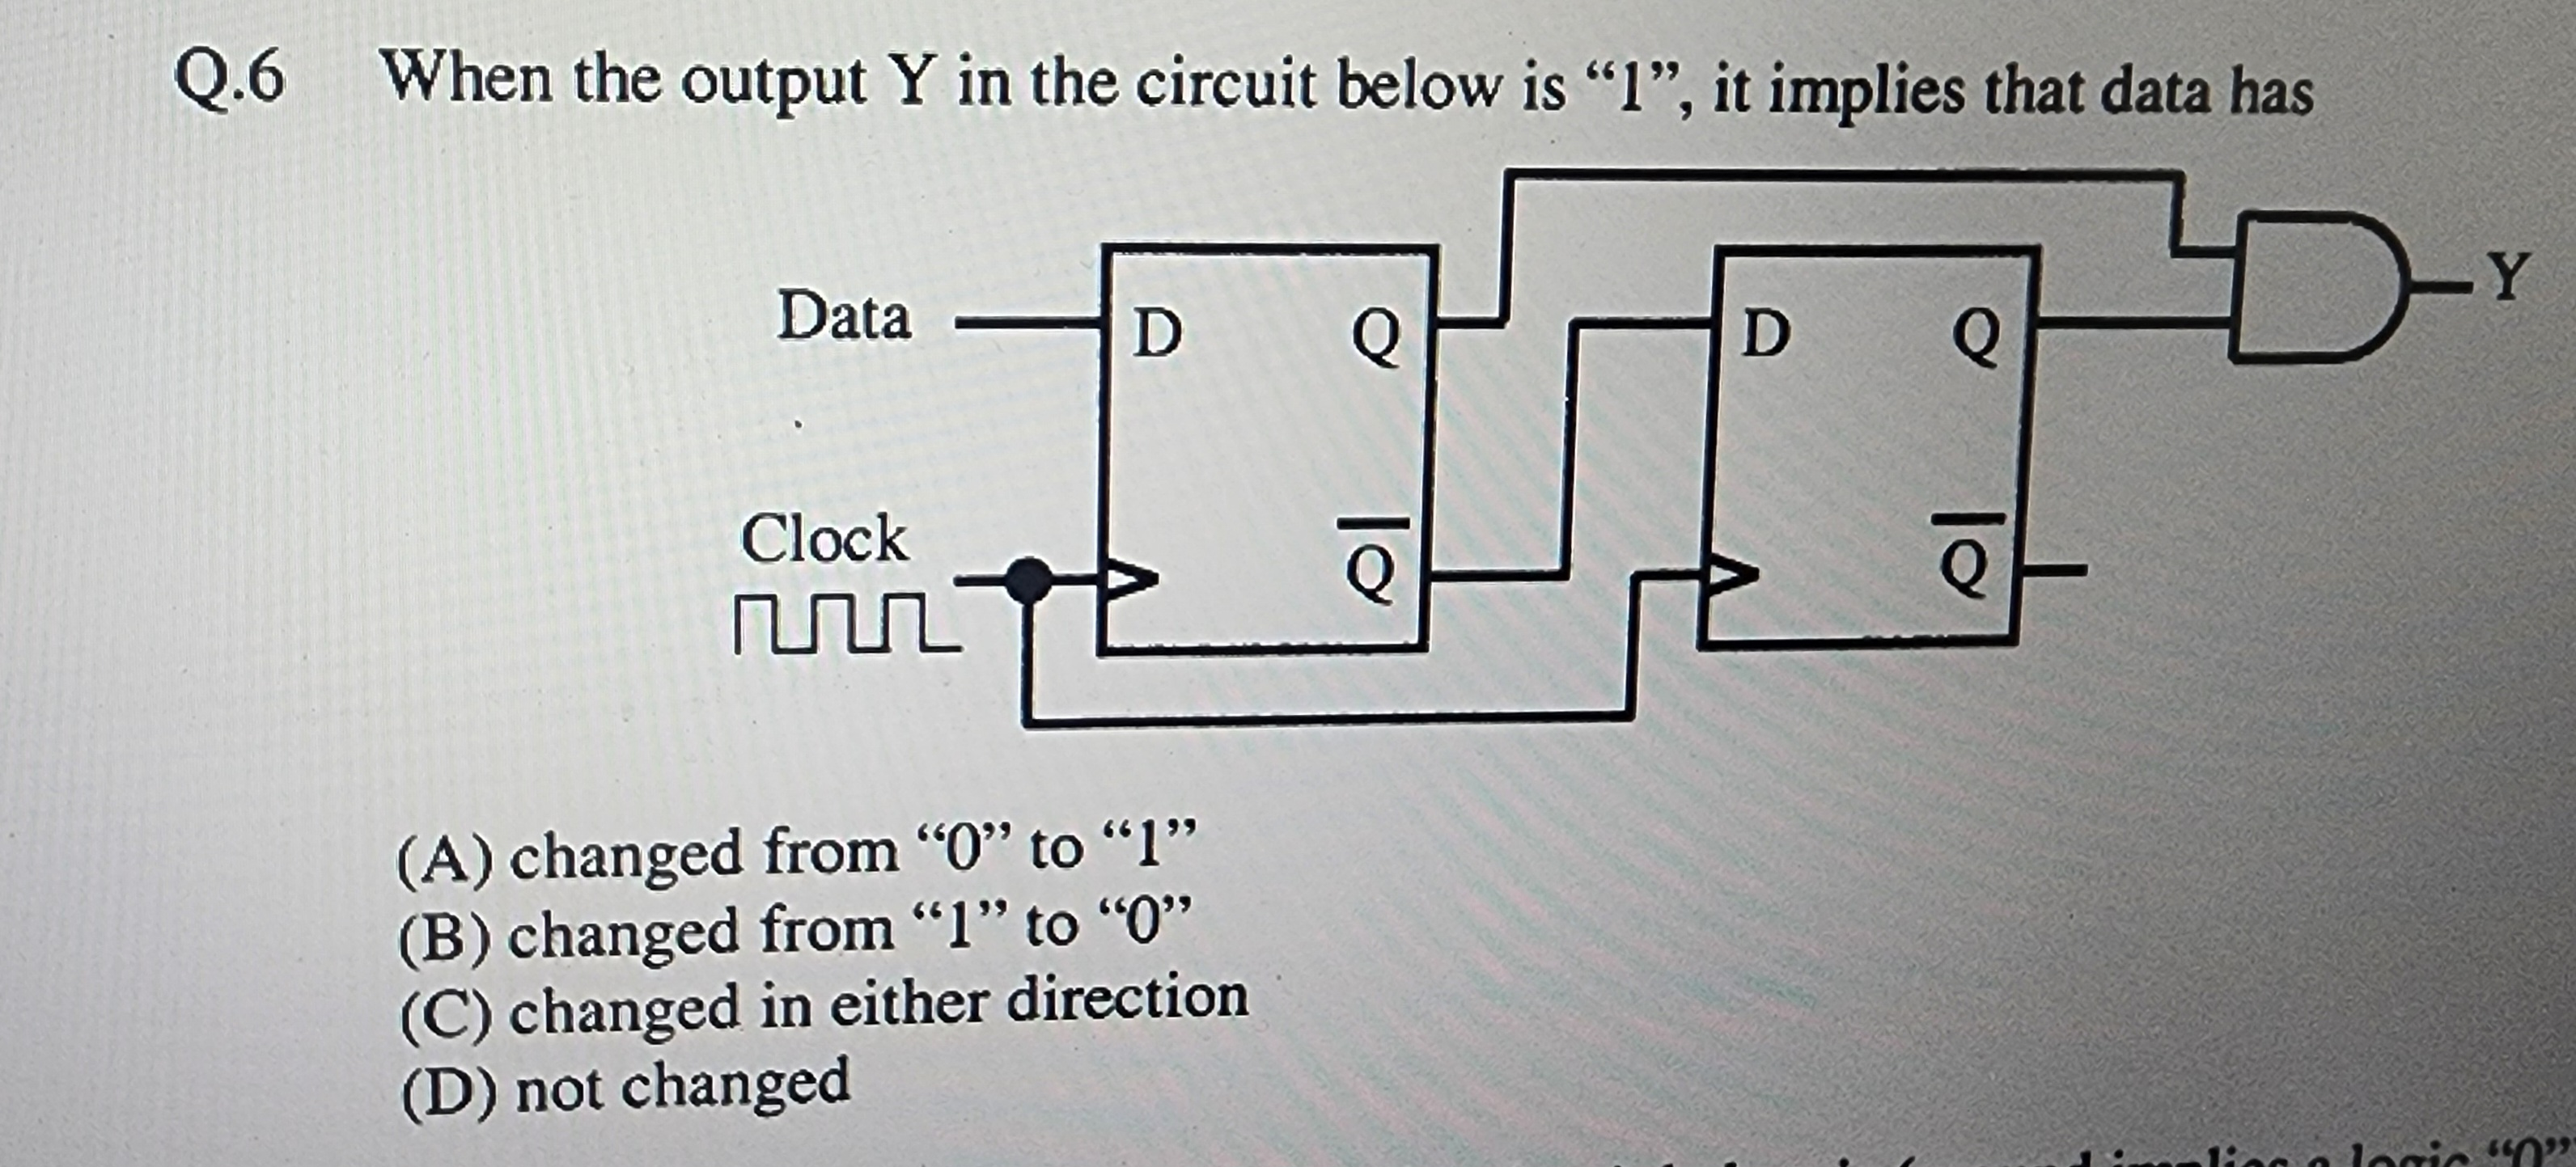
\includegraphics[width=0.7\textwidth]{aquestion.png}
    \caption{Original Q.6 from Exam Paper}
\end{figure}

\section*{Solution}

To determine when output Y in the circuit is ``1'', analyze the edge-detection logic using two D flip-flops. Y is generated by the AND of the first flip-flop's Q output and the negation of the second flip-flop's Q output:
\[
Y = Q_1 \cdot \overline{Q_2}
\]
where \( Q_1 \) is the current data and \( Q_2 \) is the previous data.

\subsection*{Truth Table}

\begin{center}
\begin{tabular}{|c|c|c|}
\hline
Q\textsubscript{2} (Previous) & Q\textsubscript{1} (Current) & Y \\
\hline
0 & 0 & 0 \\
0 & 1 & 1 \\
1 & 0 & 0 \\
1 & 1 & 0 \\
\hline
\end{tabular}
\end{center}

\subsection*{K-Map Minimization}

\[
\begin{array}{c|cc}
& Q_2=0 & Q_2=1 \\
\hline
Q_1=0 & 0 & 0 \\
Q_1=1 & 1 & 0 \\
\end{array}
\]
Thus, the minimized Boolean expression:
\[
Y = Q_1 \cdot \overline{Q_2}
\]

\section*{Implementation Steps (AVRGCC on Termux)}
\begin{enumerate}
    \item Install Termux and the necessary GCC toolchain for AVR: \texttt{pkg install clang avrgcc avrdude}
    \item Write the C code below for edge detection
    \item Compile your code: \texttt{avr-gcc -mmcu=atmega328p -o edge.bin edge.c}
    \item Flash to an AVR device using avrdude, or run with a simulator.
\end{enumerate}

\section*{Conclusion}

This circuit and corresponding software detect a rising edge on the data line, outputting ``1'' only when the data transitions from ``0'' to ``1''. The function was minimized using a Karnaugh map to \( Y = Q_1 \cdot \overline{Q_2} \). The provided C code and hardware description allow implementation with microcontrollers or logic ICs like 7474 in a FSM arrangement for precise edge detection.
\end{document}
